Figure \ref{fig:aco_block_diagram} presents a block diagram illustrating the Ant Colony Optimization metaheuristic.
The algorithm receives a weight matrix which contains the information relative to the arcs of the bipartite graph describing the problem,
aswell as other relevant data, as the duration set $D$, associated to each city $i$, of the set of nodes to be visited, $V$.
After the initialisation, and untill the termination condition is met,
the algorithm performs a cycle, in which every agent constructs a solution to the problem, 
followed by a pherormone matrix update, to reflect the search experience of each ant.

\begin{figure}[htpb]
  \centering
  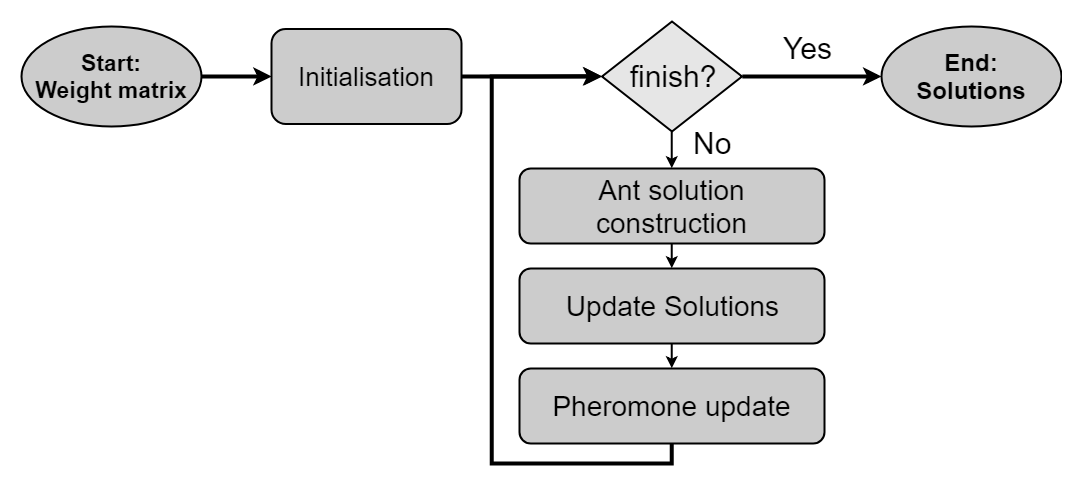
\includegraphics[width=\textwidth]{./Figures/system_implementation/aco_base.png}
  \caption{Block diagram of the Any Colony Optimization metaheuristic.}
  \label{fig:aco_block_diagram}  
\end{figure}

The initialisation of the ACO metaheuristic requires the construction of an initial pherormone matrix.
As suggested by the ACO authors \cite{aco_2},
the value of each entry of the pherormone matrix is given by equation \ref{eq:pheromone_init},
which is inversely proportional to the cost of the nearest neighbour solution, $C^{nn}$.
The initialisation of the metaheuristic also requires the definition of a variety of
algorithm specific parameters, as the number of ants $m$, the pherormone evaporation rate $\rho$,
the heuristic relative influence $\beta$, the pherormone relative influence $\alpha$,
and the exploration rate $Q_0$. 

\begin{equation}
\label{eq:pheromone_init}
  \tau_{ij}^{t} = \tau_{0} = \frac{1}{nC^{nn}}
\end{equation}

The construction process undertaken by each ant, illustrated in figure \ref{fig:aco_construction} is as follows.
First, the current time is set to a value belonging to the allowable start dates, $t \in T_0$,
and the current node is set to the start node $v_0$.
Each ant enters than an iterative cycle untill all nodes belonging to $V$ are visited.
At every step of this cycle, an ant chooses a solution component by either \textit{exploiting}
or \textit{exploring} the search space. The decision of exploiting or exploring 
depends on the algorithm parameter $Q_0$, and a pseudo-random value $q$,
calculated at run time. The selection of the solution component $j$, which identifies the next city to be visited,
is thus given by equation \ref{eq:selection_rule}.
After the selection of each solution component, it is necessary to update the time, 
incrementing it by the duration relative to the selected city.

\begin{figure}[htpb]
  \centering
  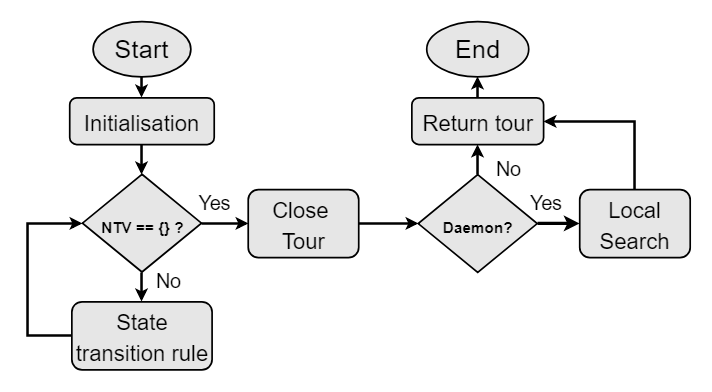
\includegraphics[width=\textwidth]{./Figures/system_implementation/aco_construction.png}
  \caption{Block diagram of the construction procedure undertaken by each ant.}
  \label{fig:aco_construction}  
\end{figure}

\begin{equation}
  \label{eq:selection_rule}
  j =  \left \{
    \begin{aligned}
      & exploitation \ (\text{eq.} \ \ref{eq:exploitation}) , && \text{if}\ q \leq Q_0 \\
      & exploration \ (\text{eq.} \ \ref{eq:exploration}), && \text{otherwise}
    \end{aligned} \right. 
\end{equation}

The exploration of the search space utilizes the so called \textit{random-proportional rule},
given by equation \ref{eq:exploitation}, which determines the next solution component 
of the ants solution. Note that $J_k(i,t)$ is the set of the solutions components 
which might be selected and form a valid solution, by an ant which is currently at city $i$ at time $t$.
In its turn, the exploration is given by equation \ref{eq:exploration},
and $p_a(i,j,t)$ represents the probability of ant $a$,
which is currently at the node $i$ at time $t$, selecting $j$ as the next node to visit.
In the presented equations, $\eta$ is the inverse of the weight matrix value.

\begin{equation}
  \label{eq:exploitation}
    arg max_{j \in J_k(i,t)} {[\tau(i,j,t)][\eta(i,j,t)]^\beta}
\end{equation}


\begin{equation}
\label{eq:exploration}
  p_a(i,j,t) =  \left \{
    \begin{aligned}
      & \frac{[\tau(i,j,t)][\eta(i,j,t)]^\beta}{\sum_{u \in J_k(i,t)}[\tau(i,u,t)][\eta(i,u,t)]^\beta}, && \text{if}\ j \in J_k(i,t) \\
      &0, && \text{otherwise}
    \end{aligned} \right. 
\end{equation}

Follwing the iterative construction procedure, an uncomplete solution is available.
To complete this solution, it is necessary to add an extra solution component, which connects the last visited node,
to the return node, $v_{n+1}$.

Having a complete solution, it is possible to perform \textit{Daemon Actions}, or in other words, try to improve 
the constructed solution using a local search algorithm. The execution of this step is optional,
and is set by a parameter algorithm at the initialization of the procedure.
The selection of a local search algorithm is usually problem specific,
and for the Traveling Salesman Problem, one of the most used local search procedures is the $k$-opt exchange.
During the development of this work, the 2-opt procedure was utilized.

The mainstream success of the Ant Colony Optimization in the multiple areas in which it was applied,
is due to its ability to \textit{guide} the agents to good solutions.
While the construction of each solution follows a pseudo-random rule,
the overall quality of this solution is used to bias the search towards the search space around this solution.
This achieved by the global pheromone update, given by equation \ref{eq:global_update}.


\begin{equation}
\label{eq:global_update}
  \tau_{ijt} = (1-\rho)\tau_{ijt} + \sum_{s \in S_{upd} | c_{ijt} \in s} g(s)
\end{equation}

The global pheromone update is a proccess in which, at every step of the algorithm,
all entries of the pheromone matrix are updated, by the so called pheromone \textit{evaporation} and \textit{depositation}.
Pheromone evaporation is a method used to avoid getting stuck in sub-optimal solutions,
while pheromone deposition intends to induce the exploration of the search space around good solutions,
by incrementing the pheromone values of the solution components belonging to a set $S_{upd}$.
The set $S_{upd}$ is usually a subset of the solutions constructed at the current iterative step,
$S_{upd} \subset S_{iter}$.
Furthermore, the set $S_{upd}$ includes the best global solution $S_{best}$,
and this work follows the elitist ant rule, which defines that pheromone deposition on the solution 
components beloning to $S_{best}$ is actually higher than those of the other solutions in $S_{upd}$.
In equation \ref{eq:global_update}, $g(): S \rightarrow \mathcal{R}^+$ is a function such that $f(s) < f(s^{'}) \Rightarrow g(s) \geq g(s^{'})$.
It is common set $g()$ to be inversely proportional to the objective function $f()$.
Thus, the inversely proportional constant for $g$ is set to $1$ for all solution components in $S_{upd}$,
and to a higher value for $S_{best}$, 3 in this case, due to the elitist ant rule.






